\documentclass[12pt,letterpaper]{article}
\usepackage{graphicx,textcomp}
\usepackage{natbib}
\usepackage{setspace}
\usepackage{fullpage}
\usepackage{color}
\usepackage[reqno]{amsmath}
\usepackage{amsthm}
\usepackage{fancyvrb}
\usepackage{amssymb,enumerate}
\usepackage[all]{xy}
\usepackage{endnotes}
\usepackage{lscape}
\newtheorem{com}{Comment}
\usepackage{float}
\usepackage{hyperref}
\newtheorem{lem} {Lemma}
\newtheorem{prop}{Proposition}
\newtheorem{thm}{Theorem}
\newtheorem{defn}{Definition}
\newtheorem{cor}{Corollary}
\newtheorem{obs}{Observation}
\usepackage[compact]{titlesec}
\usepackage{dcolumn}
\usepackage{tikz}
\usetikzlibrary{arrows}
\usepackage{multirow}
\usepackage{xcolor}
\newcolumntype{.}{D{.}{.}{-1}}
\newcolumntype{d}[1]{D{.}{.}{#1}}
\definecolor{light-gray}{gray}{0.65}
\usepackage{url}
\usepackage{listings}
\usepackage{color}

\definecolor{codegreen}{rgb}{0,0.6,0}
\definecolor{codegray}{rgb}{0.5,0.5,0.5}
\definecolor{codepurple}{rgb}{0.58,0,0.82}
\definecolor{backcolour}{rgb}{0.95,0.95,0.92}

\lstdefinestyle{mystyle}{
	backgroundcolor=\color{backcolour},   
	commentstyle=\color{codegreen},
	keywordstyle=\color{magenta},
	numberstyle=\tiny\color{codegray},
	stringstyle=\color{codepurple},
	basicstyle=\footnotesize,
	breakatwhitespace=false,         
	breaklines=true,                 
	captionpos=b,                    
	keepspaces=true,                 
	numbers=left,                    
	numbersep=5pt,                  
	showspaces=false,                
	showstringspaces=false,
	showtabs=false,                  
	tabsize=2
}
\lstset{style=mystyle}
\newcommand{\Sref}[1]{Section~\ref{#1}}
\newtheorem{hyp}{Hypothesis}

\title{Problem Set 4}
\date{Due: April 12, 2024}
\author{Applied Stats II}


\begin{document}
	\maketitle
	\section*{Instructions}
	\begin{itemize}
	\item Please show your work! You may lose points by simply writing in the answer. If the problem requires you to execute commands in \texttt{R}, please include the code you used to get your answers. Please also include the \texttt{.R} file that contains your code. If you are not sure if work needs to be shown for a particular problem, please ask.
	\item Your homework should be submitted electronically on GitHub in \texttt{.pdf} form.
	\item This problem set is due before 23:59 on Friday April 12, 2024. No late assignments will be accepted.

	\end{itemize}

	\vspace{.25cm}
\section*{Question 1}
\vspace{.25cm}
\noindent We're interested in modeling the historical causes of child mortality. We have data from 26855 children born in Skellefteå, Sweden from 1850 to 1884. Using the "child" dataset in the \texttt{eha} library, fit a Cox Proportional Hazard model using mother's age and infant's gender as covariates. Present and interpret the output.

	\noindent \textbf{Codes as below:}
    \lstinputlisting[language=R, firstline=47, lastline=57]{PS4.R}% \vspace{.25cm}
    \vspace{2.75cm}
    
    \noindent \textbf{Summary output:}
    % Table created by stargazer v.5.2.3 by Marek Hlavac, Social Policy Institute. E-mail: marek.hlavac at gmail.com% Date and time: Wed, Apr 10, 2024 - 21:40:52
    \begin{table}[!htbp] \centering   \caption{}   \label{} 
    	\begin{tabular}{@{\extracolsep{5pt}}lc} \\[-1.8ex]\hline \hline \\[-1.8ex]  & \multicolumn{1}{c}{\textit{Dependent variable:}} \\ \cline{2-2} \\[-1.8ex] & child\_surv \\ \hline \\[-1.8ex]  m.age & 0.008$^{***}$ \\   & (0.002) \\   & \\  sexfemale & $-$0.082$^{***}$ \\   & (0.027) \\   & \\ \hline \\[-1.8ex] Observations & 26,574 \\ R$^{2}$ & 0.001 \\ Max. Possible R$^{2}$ & 0.986 \\ Log Likelihood & $-$56,503.480 \\ Wald Test & 22.520$^{***}$ (df = 2) \\ LR Test & 22.518$^{***}$ (df = 2) \\ Score (Logrank) Test & 22.530$^{***}$ (df = 2) \\ \hline \hline \\[-1.8ex] \textit{Note:}  & \multicolumn{1}{r}{$^{*}$p$<$0.1; $^{**}$p$<$0.05; $^{***}$p$<$0.01} \\ 
    	\end{tabular} 
    \end{table} 

	
	\noindent \textbf{Interpretation:} 
	\\1. m.age (mother's age): The coefficient is 0.008 (***). This indicates that for every one-year increase in mother's age, the risk of infant survival increases by a factor of 1.008 on average. The three asterisks denote that this result is highly statistically significant (p $<$ 0.01).
	\\2. sexfemale (infant's gender): The coefficient is -0.082. This suggests that compared to male infants, the survival risk of female infants decreases by a factor of 0.082 on average, or in other words. Similarly, the three asterisks denote that this result is highly statistically significant (p $<$ 0.01).
	\\\\In summary, increasing mother's age is associated with an increase in infant survival risk, while female infants have a higher survival risk compared to male infants.
	
	 \vspace{2.0cm}
	\noindent \textbf{Model Evaluation and Visualization:}
	\lstinputlisting[language=R, firstline=61, lastline=66]{PS4.R}
	
	\noindent \textbf{Output:}
	% Table created by stargazer v.5.2.3 by Marek Hlavac, Social Policy Institute. E-mail: marek.hlavac at gmail.com% Date and time: Wed, Apr 10, 2024 - 21:40:52
	\begin{table}[!htbp] \centering   \caption{}   \label{} 
		\begin{tabular}{@{\extracolsep{5pt}}lccccc} \\[-1.8ex]\hline \hline \\[-1.8ex] Statistic & \multicolumn{1}{c}{N} & \multicolumn{1}{c}{Mean} & \multicolumn{1}{c}{St. Dev.} & \multicolumn{1}{c}{Min} & \multicolumn{1}{c}{Max} \\ \hline \\[-1.8ex] Df & 2 & 1.000 & 0.000 & 1 & 1 \\ AIC & 3 & 113,017.100 & 5.528 & 113,011.000 & 113,021.800 \\ LRT & 2 & 11.130 & 2.355 & 9.465 & 12.795 \\ Pr(\textgreater Chi) & 2 & 0.001 & 0.001 & 0.0003 & 0.002 \\ \hline \\[-1.8ex] 
		\end{tabular} 
	\end{table}
	
	\begin{figure}[htbp]
		\centering
		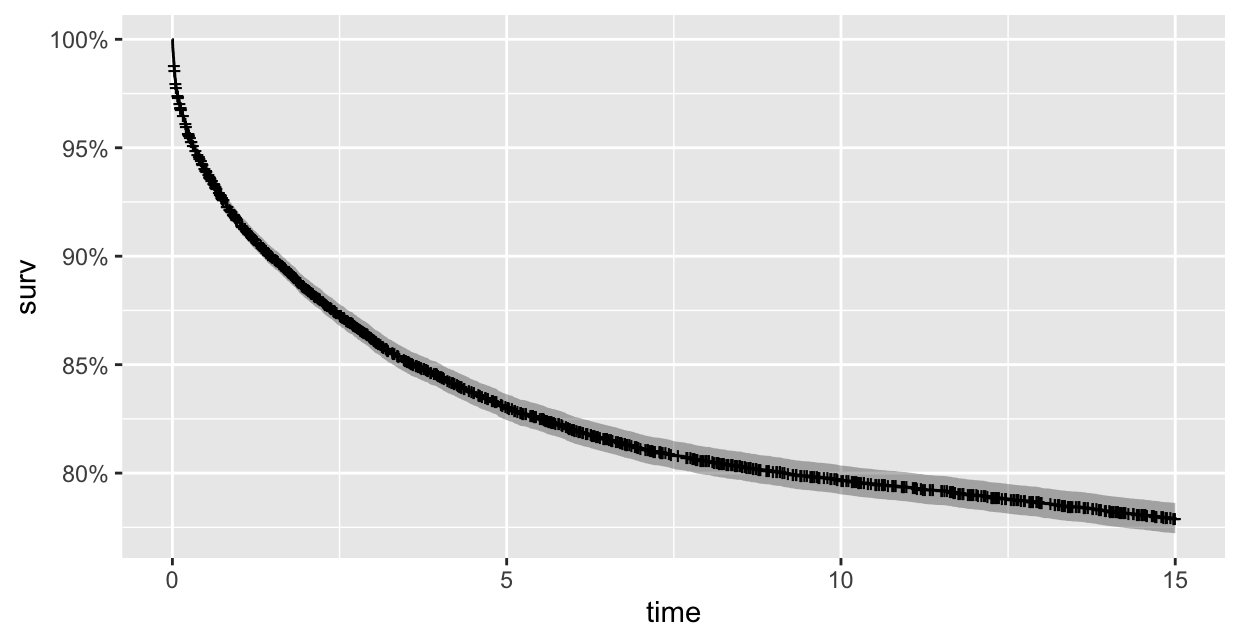
\includegraphics[width=0.8\textwidth]{plot.png}
		\label{fig:my_image}
	\end{figure}
	
	\noindent \textbf{Interpretation:}
	\\In the assessment results of the Cox Proportional Hazard model, the statistical significance p-values of the model are all less than 0.05, indicating that the variables in the model have a significant impact on survival time.
	\\The survival curve plot displays estimated survival probabilities at specific time points. For example, at the 15-year timestamp, the survival probability drops to approximately 75%.
	
\end{document}


